\documentclass[12pt,a4paper]{article}

\usepackage[utf8]{inputenc}
\usepackage[T1]{fontenc}
\usepackage[french]{babel}
\usepackage{lmodern}
\usepackage[a4paper,margin=2.5cm]{geometry}
\usepackage{xcolor}
\usepackage{hyperref}
\usepackage{graphicx}
\usepackage{booktabs}
\usepackage{enumitem}
\usepackage{listings}

\hypersetup{
  colorlinks=true,
  linkcolor=blue,
  urlcolor=blue,
  pdftitle={Compte rendu - API Iris avec Redis},
  pdfauthor={},
}

\definecolor{codegray}{gray}{0.95}
\lstset{
  basicstyle=\ttfamily\small,
  backgroundcolor=\color{codegray},
  frame=single,
  breaklines=true,
  columns=fullflexible,
  showstringspaces=false,
  language=bash
}

\begin{document}

\begin{titlepage}
  \centering
  \vspace*{2cm}

  {\Large\textbf{Compte rendu de projet}\par}
  \vspace{1.5cm}

  {\huge\bfseries API Iris conteneurisée\par}
  \vspace{0.4cm}
  {\huge\bfseries avec mémoire Redis\par}

  \vfill

  \begin{tabular}{rl}
    \textbf{Étudiant :} & Aymane El Yamani \\
    \textbf{Professeur :} & Mohamed Ameksa
  \end{tabular}

  \vfill

  {\large Année universitaire 2026\par}
  \vspace{0.5cm}
  {\large \today\par}
\end{titlepage}

\tableofcontents
\newpage

\section{Objectif du projet}

L'objectif du projet est de reprendre une API de prédiction basée sur le jeu de
données Iris et de lui ajouter une mémoire. L'API effectue les prédictions,
tandis que Redis compte le nombre total de prédictions réalisées.

Le projet met en œuvre :
\begin{itemize}[itemsep=0.2em]
  \item une API HTTP développée avec FastAPI ;
  \item un modèle de régression logistique entraîné sur Iris ;
  \item une communication entre conteneurs avec Docker Compose ;
  \item un compteur persistant dans Redis grâce à un volume nommé.
\end{itemize}

\section{Architecture}

L'application est composée de deux services :
\begin{description}[style=nextline]
  \item[\texttt{api}] Conteneur Python qui expose l'API sur le port 8000.
  Le modèle Iris est chargé et entraîné au démarrage du processus.
  \item[\texttt{base}] Conteneur Redis basé sur l'image
  \texttt{redis:7-alpine}. Le mode AOF est activé afin de conserver les
  écritures sur le volume \texttt{redis-data}.
\end{description}

Le nom DNS \texttt{base} est utilisé par l'API pour joindre Redis sur le port
6379. Le service \texttt{api} dépend du healthcheck Redis et ne démarre qu'une
fois que Redis répond correctement à la commande \texttt{PING}.

\section{Implémentation de l'API}

Le fichier principal est \texttt{src/app.py}. Le modèle est entraîné à partir
de \texttt{load\_iris} avec une régression logistique. Le code correspondant
dans le projet est présenté ci-dessous :

\begin{figure}[ht]
  \centering
  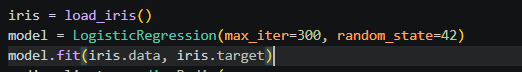
\includegraphics[width=0.92\textwidth]{images/01_load_iris.png}
  \caption{Chargement des données Iris et entraînement du modèle}
\end{figure}

La requête de prédiction doit contenir exactement quatre mesures. La définition
réelle de \texttt{PredictionRequest} est illustrée ci-dessous :

\begin{figure}[ht]
  \centering
  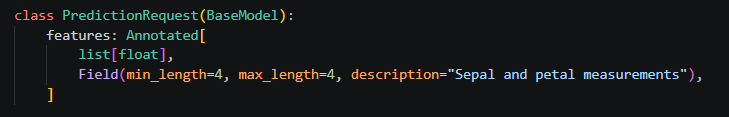
\includegraphics[width=0.92\textwidth]{images/02_PredictionRequest.png}
  \caption{Validation des données reçues par l'API}
\end{figure}

Lorsqu'une prédiction réussit, l'API appelle \texttt{INCR} sur la clé Redis
\texttt{predictions}. Cette opération est atomique et renvoie directement la
nouvelle valeur du compteur.

\subsection{Endpoints}

\begin{center}
\begin{tabular}{lll}
\toprule
\textbf{Méthode} & \textbf{Route} & \textbf{Rôle} \\
\midrule
\texttt{GET} & \texttt{/health} & Vérifie que Redis est accessible \\
\texttt{POST} & \texttt{/predict} & Prédit une espèce et incrémente le compteur \\
\texttt{GET} & \texttt{/stats} & Retourne le nombre de prédictions \\
\bottomrule
\end{tabular}
\end{center}

Exemple de requête :

\begin{lstlisting}
curl -X POST http://localhost:8000/predict ^
  -H "Content-Type: application/json" ^
  -d "{\"features\":[5.1,3.5,1.4,0.2]}"
\end{lstlisting}

Réponse observée :

\begin{lstlisting}
{"prediction":0,"species":"setosa","count":1}
\end{lstlisting}

La route \texttt{/stats} renvoie ensuite :

\begin{lstlisting}
{"predictions":1}
\end{lstlisting}

Si Redis est indisponible, l'API retourne une erreur HTTP 503 au lieu de
simuler un compteur ou de masquer l'erreur.

\section{Conteneurisation}

Le \texttt{Dockerfile} utilise \texttt{python:3.12-slim}. Les dépendances sont
installées depuis \texttt{requirements.txt}, puis seul le fichier
\texttt{src/app.py} est copié dans l'image. L'application s'exécute avec
l'utilisateur non privilégié \texttt{appuser}.

La commande de démarrage est :

\begin{lstlisting}
uvicorn app:app --host 0.0.0.0 --port 8000
\end{lstlisting}

Le nom \texttt{app:app} correspond au fichier \texttt{app.py} et à l'objet
FastAPI nommé \texttt{app}.

\section{Orchestration avec Docker Compose}

Le fichier \texttt{docker-compose.yml} définit les deux services et le volume :

\begin{figure}[ht]
  \centering
  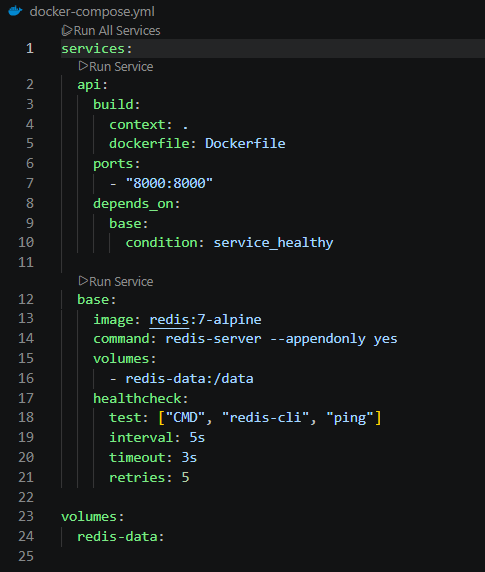
\includegraphics[width=0.92\textwidth]{images/03_docker-compose.yml.png}
  \caption{Configuration Docker Compose des services API et Redis}
\end{figure}

Avant le démarrage, la configuration a été vérifiée avec :

\begin{lstlisting}
docker compose config
\end{lstlisting}

Cette commande a confirmé que les services, le healthcheck, le réseau et le
volume étaient correctement interprétés par Compose.

\section{Tests et résultats}

L'application a été construite et démarrée avec :

\begin{lstlisting}
docker compose up --build
\end{lstlisting}

Le service Redis a répondu \texttt{PONG} à son healthcheck, puis Uvicorn a
indiqué que l'API écoutait sur \texttt{0.0.0.0:8000}.

Trois requêtes identiques sur \texttt{/predict} ont renvoyé successivement les
compteurs 1, 2 et 3. Le résultat de \texttt{/stats} était :

\begin{lstlisting}
{"predictions":3}
\end{lstlisting}

\subsection{Effet de \texttt{docker compose down}}

La commande :

\begin{lstlisting}
docker compose down
docker compose up -d
\end{lstlisting}

supprime les conteneurs et le réseau, mais conserve le volume nommé. Après le
redémarrage, \texttt{/stats} a donc renvoyé :

\begin{lstlisting}
{"predictions":3}
\end{lstlisting}

Le compteur a bien survécu à l'arrêt normal de l'application.

\subsection{Effet de \texttt{docker compose down -v}}

La commande :

\begin{lstlisting}
docker compose down -v
docker compose up -d
\end{lstlisting}

supprime également le volume \texttt{redis-data}. Redis redémarre alors avec
une base vide et \texttt{/stats} renvoie :

\begin{lstlisting}
{"predictions":0}
\end{lstlisting}

\section{Bilan}

Le projet répond à l'objectif demandé : la prédiction reste assurée par l'API
et Redis fournit une mémoire externe pour compter les appels. La persistance
dépend directement de la durée de vie du volume Docker :
\begin{itemize}
  \item \texttt{down} conserve les données ;
  \item \texttt{down -v} les supprime.
\end{itemize}

La séparation entre l'API et Redis permet également de redémarrer le service
web sans perdre l'état du compteur, tout en conservant une configuration
reproductible avec Docker Compose.

\end{document}
